\clearpage
\subsection{屏幕外的倒影}
\label{sec:mirror}

相机正对一面镜子，灯牌架在相机背后。打开 SSR，镜面上的像素可以沿反射方向去查本帧画好的颜色。但整张图里没有一个像素画过灯牌，屏幕上就无从查到它的条纹。要画出镜子里的灯牌，可以从这个像素对应的镜面位置出发，沿反射方向去找房间里实际摆放的物体。

\begin{center}
\begin{tikzpicture}[x=1cm,y=1cm,font=\small,>=stealth]
\foreach \k/\heading in {0/镜子看得到灯牌,1/挡板遮住灯牌}{
  \begin{scope}[xshift=\k*7.85cm]
  \filldraw[rounded corners=2mm,fill=shade!75,draw=quiet!30] (0,0) rectangle (7.55,4.9);
  \node[anchor=west,font=\bfseries] at (.23,4.56) {\heading};
  \draw[teal!70!black,line width=1.8pt] (.7,3.65)--(6.7,3.65);
  \node[anchor=south east,text=teal!60!black] at (6.65,3.65) {镜面};
  \fill[teal!70!black] (2.60,3.65) circle (2.1pt);
  \draw[quiet!60,dashed] (2.6,3.62)--(2.6,2.47);
  \node[text=quiet,anchor=north] at (2.6,2.48) {法线};
  \draw[ink,thick,->] (1.45,1.85)--(2.58,3.61);
  \fill[ink] (1.45,1.85) circle (2pt);
  \node[anchor=north east] at (1.65,1.83) {相机};
  \draw[wine,line width=3pt] (4.01,.77)--(5.03,.77);
  \node[text=wine,anchor=north] at (4.52,.72) {条纹灯牌};
  \ifnum\k=0
    \draw[wine,thick,->] (2.62,3.62)--(4.43,.79);
  \else
    \draw[quiet!55,dashed] (3.67,1.98)--(4.45,.78);
    \draw[quiet,line width=3pt] (3.31,1.98)--(4.14,1.98);
    \node[text=quiet,anchor=west] at (4.22,1.98) {挡板};
    \draw[wine,thick,->] (2.62,3.62)--(3.63,2.02);
  \fi
  \end{scope}
}
\end{tikzpicture}
\end{center}
{\small\color{quiet}项目绘制的俯视图。按程序查找物体的方向读箭头：黑线从相机走到镜面，红线从镜面走到第一个交点。右图的虚线表示挡板后面的路，灯牌在这里照不进镜子。\par}

先看左图。画一条垂直于镜面的线，标作单位法线 $n$。从相机走到镜面的单位方向记为 $d$。把 $d$ 分成两部分，一部分沿着镜面向右，另一部分垂直镜面向里。反射后仍向右走，原本向里的那部分要改成向外。这一部分是 $(d\cdot n)n$，从 $d$ 减去它一次只够把它消掉，再减一次才会反向。于是从镜面出发的方向为
\[
    r=d-2(d\cdot n)n .
\]
例如用“向右、远离镜面”作两个坐标方向，来路 $d=(0.6,-0.8)$ 就会变成 $r=(0.6,0.8)$。着色器里的 $v$ 从表面指向相机，正好与来路相反，因此理想镜面的代码是 \texttt{reflect(-v,n)}。粗糙度为零时，\texttt{sampleReflection} 每次都取这条方向。粗糙表面则按前文的 GGX 分布选取小镜子的法线 $h$，再求 \texttt{reflect(-v,h)}。采到的方向散开，灯条的轮廓也会变宽。\href{https://pbr-book.org/4ed/Reflection_Models/Specular_Reflection_and_Transmission}{PBRT 第四版 §9.3.3，图 9.6、9.7}

右图里，沿同一方向既能碰到挡板，也能碰到灯牌。把起点记为 $P$，离镜面 $t$ 个场景单位的点就是 $P+t\,r$。查找只走到设置中的反射距离，默认是 12 个场景单位。范围内各个不透明表面当中，最小的正数 $t$ 给出挡板。在这个交点取颜色，即使挡板完全是黑色，也要把黑色留在倒影里。用“颜色够不够亮”判断有没有碰到东西，会让远处的灯牌或天空穿过挡板。

方向还不能决定镜子有多亮。理想的白金属可以把这条方向上的光全部反回来。对于项目里的光滑非金属材质，正对表面时镜面反射约占入射光的 4\%，朝侧面看时这个比例会增大。着色器用菲涅耳项 $F$ 表示这个比例。镜子照到天空时，粗糙度为零就从环境图最清晰的那层取色，再乘 $F$。

在 \texttt{Mirror-Studio} 里，镜面位于 $z=0$。相机的水平位置是 $x=-0.62,\ z=3$，灯牌中心在 $x=1.75,\ z=4.8$。想象把灯牌移到镜后一样远的地方，虚像就在 $z=-4.8$。从相机向虚像画直线，走过全程的 $3/7.8$ 就会与镜面相交。交点的横向位置是 $-0.62+(1.75+0.62)\times3/7.8\approx0.29$。从这里往真实灯牌连线，走到 $z=2.55$ 时，横向位置约为 $1.07$。把挡板中心摆在这里，就能遮住镜中的灯条，同时给相机留出看镜面的视线。\href{run:../../RedflagForge/assets/scenes/Mirror-Studio.redflag}{示例场景}\quad\href{run:../../tests/check_scene_reflections.py}{挡板的位置与截帧}

\clearpage
\subsection{倒影中的颜色}

组合光照先算出相机能直接看到的物体颜色，再算倒影。能够从屏幕上查到立柱时，直接读立柱那个像素的颜色。打开「实时效果」里 SSR 下的「屏幕外反射」后，射线在屏幕上找不到交点，还可以查询房间里的三角形。CPU 在加载几何时已经把附近的三角形分组，给每组套上包围盒。GPU 从镜面出发，光线没穿过的盒子可以整组略过。这次计算沿用间接光照的这份场景数据。

\noindent{\small\color{quiet}按计算着色器整理的伪代码\quad
\href{run:../../Redflag/src/Redflag/Renderer/ScreenSpace/Shaders/StochasticSSR.comp}{\texttt{StochasticSSR.comp}，\texttt{main}}}\par\nopagebreak
\begin{lstlisting}[escapeinside={(*@}{@*)}]
r, weight = sampleReflection(normal, view, roughness)
if hitScreen(r):
    incoming = sceneColor[hitPixel]    (*@{\footnotesize\color{quiet}这个像素已经算过光照。}@*)
else if traceScene and hitScene(r):
    incoming = shade(hit, -r)          (*@{\footnotesize\color{quiet}从交点朝镜子看，算它送来的光。}@*)
else:
    return base + environmentReflection
return base + incoming * weight        (*@{\footnotesize\color{quiet}镜面把入射光中的这一份反射到相机。}@*)
\end{lstlisting}

镜子照到灯牌时，交点给出灯牌上的纹理坐标。顺着坐标找到发光贴图上的条纹，把纹素从 sRGB 转为线性颜色，再乘材质的发光颜色和强度，就能分清亮条、暗条和黑边。若照到一面普通墙，还要看哪些点光源或方向光能照到它。此时视线从墙指向镜子，高光的方向也按这条视线计算。启用 DDGI 后，墙面还能从附近的探针取到反射来的光。编辑器在探针算完第一轮或读入烘焙文件后才使用这份数据。镜子前什么都没碰到时，已启用的镜面环境光可以提供远景。环境图按方向取色，花纹随位置改变的近处灯牌需要前面的交点才能画准。

这些计算可在 \href{run:../../Redflag/src/Redflag/Renderer/ScreenSpace/Shaders/SceneReflection.glsl}{\texttt{SceneReflection.glsl} 的 \texttt{sceneReflection}} 中找到。交点取三角形本身的法线，法线贴图刻出的细纹可能在倒影里变平。计算会略过标成半透明的玻璃。若叶片使用透明度裁剪，射线会在交点读取贴图的透明度，遇到孔隙便继续查找后面的物体。镜子里出现第二面镜子时，只计算第二面镜子自身的材质和照明。

在 GPU 上读一次屏幕颜色很直接，沿场景查找还需读包围盒、三角形和材质。AMD 的 FidelityFX 示例也利用两种查询各自能看到的物体，并用屏幕分块和降噪控制工作量。本项目由 Vulkan 计算着色器沿包围盒查找，同一条反射光线找到屏幕颜色就结束查找。屏幕颜色来自主相机的视角，因此把带窄高光的物体转过屏幕边缘时，两种方法算出的高光仍可能不同。\href{https://gpuopen.com/manuals/fidelityfx_sdk/samples/hybrid-reflections/}{AMD 示例说明}\quad\href{https://github.com/GPUOpen-LibrariesAndSDKs/FidelityFX-SDK/blob/v1.1.4/samples/hybridreflections/shaders/Intersect.hlsl}{SDK 1.1.4 源码}\quad
\href{https://gpuopen.com/download/GDC_Performant_Reflective_Beauty_Hybrid_Ray_Traced_Reflections_In_Far_Cry_6.pdf}{GDC 2022 讲义，第 74--77 页}

\pair[.43\linewidth]{profiling/scene-reflections/bathroom-screen.png}{只开 SSR}{profiling/scene-reflections/bathroom-scene.png}{加上屏幕外反射}
{\small\color{quiet}RTXGI Bathroom 同机位，第 24 帧，RenderDoc 回放，$320\times205$。看洗手盆上方的圆镜：右图能看到身后墙砖的明暗交界，镜面和粗糙的地面仍有颗粒。\par}

\clearpage
\subsection{灯条与挡板的实测}

回到 \texttt{Mirror-Studio}，用相同机位捕获第 24 帧。左图里镜面上有两处点光源的高光，但灯牌没有出现。右图里多出三条橙色灯带，后方的墙也进入倒影。再把绿色挡板放到镜面和灯牌的连线上，镜子里原本最亮的区域就变成绿色。三次都保留 SSR，改动的是从场景中查找物体的开关和挡板的位置。

\pair{profiling/scene-reflections/mirror-screen.png}{仅从屏幕取色}{profiling/scene-reflections/mirror-scene.png}{从场景中找到灯牌}
\begin{center}
  \begin{minipage}[c]{.48\linewidth}\centering
    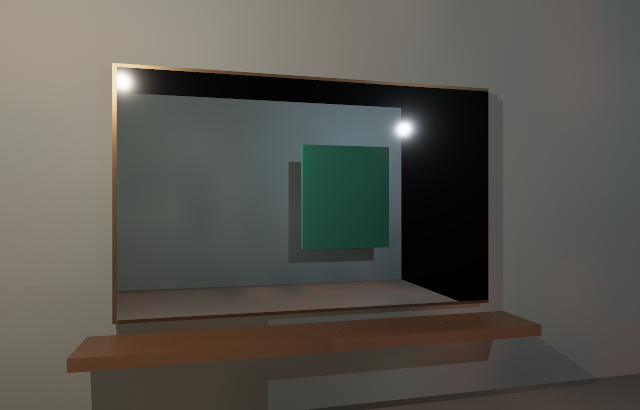
\includegraphics[width=\linewidth]{../../../output/profiling/scene-reflections/mirror-blocked.png}\\[-2pt]
    {\small 在镜子和灯牌之间放入挡板}
  \end{minipage}\hfill
  \begin{minipage}[c]{.48\linewidth}\centering
  {\small 加入屏幕外反射后，镜中各处的读数}\par\smallskip
  \small\begin{tabular}{@{}lrr@{}}
    \toprule 取样处 & 红通道 & 绿通道\\\midrule
    亮条中心 & \measured{mirror-white-r} & \measured{mirror-white-g}\\
    灰条中心 & \measured{mirror-gray-r} & \measured{mirror-gray-g}\\
    黑色间隔 & \measured{mirror-black-r} & \measured{mirror-black-g}\\
    绿色挡板 & \measured{mirror-board-r} & \measured{mirror-board-g}\\\bottomrule
  \end{tabular}
  \end{minipage}
\end{center}
{\small\color{quiet}RenderDoc 1.47 回放，$640\times410$，原图使用编辑器的亮度映射。表中每项取交点附近 $3\times3$ 个像素的中位数，读取反射计算前后的线性颜色之差，所以数值可以大于 1。最后一行仍取第一行的位置。\par}

灯牌中间那条在 8 位贴图里取的是灰色 128。把 sRGB 转回线性亮度，理论上它发出的光约为白色的 $0.216$ 倍。灯牌表面同时也会反射房间的光，可以用不发光的黑色间隔估计这部分。用上表的红通道扣除它，得到 $(\measured{mirror-gray-r}-\measured{mirror-black-r})/(\measured{mirror-white-r}-\measured{mirror-black-r})\approx\measured{mirror-stripe-ratio}$。这样既检查了射线找到的物体，也检查了取到哪条花纹、它应该有多亮。

只开 SSR 时，这三个位置的反射增量全部为零。放入挡板后，亮条原处的红通道降到 \measured{mirror-board-r}，绿通道仍有 \measured{mirror-board-g}，镜子收到了挡板送来的光。单帧可以看出颜色是否正确。要判断同一像素的亮度会不会来回跳动，还要把它在不同帧的值取出来比较。\href{run:../profiling/scene-reflections/frames.json}{五次截帧的图像、绘制事件与原始读数}
\clearpage
\subsection{理想镜面的边缘}

灯条的颜色对了，把镜中的灯牌放大，边缘却像撒着一层亮砂。相机和灯牌都没动，镜面材质的粗糙度也已经调到零。对于这样的镜面，表面法线和视线都固定，每帧应沿同一个方向取色。可以先查反射方向是否真的固定，再去调整 TAA。

\begin{center}\small
\begin{tabular}{@{}c@{\hspace{12mm}}c@{}}
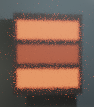
\includegraphics[width=.28\linewidth]{../../../output/profiling/scene-reflections/mirror-edge-before.png} &

\includegraphics[width=.28\linewidth]{../../../output/profiling/scene-reflections/mirror-edge-after.png}\\[-2pt]
旧版仍然随机选方向 & 粗糙度为零时用镜面方向
\end{tabular}\end{center}
{\small\color{quiet}从两次 RenderDoc 回放的同一屏幕位置裁出灯牌，各取第 24 帧的 $94\times107$ 个像素。两次都用粗糙度为零的镜子，使用同一份烘焙探针。可对照灯条内部和四边，亮砂主要出现在亮暗交界处。\par}

旧着色器用 $a=\max(0.002,\,\text{roughness}^2)$ 决定抽样范围。它本来用来画有粗糙度的材质。即使把粗糙度调到零，旧代码仍取 $a=0.002$，每帧抽出的小镜子朝向都会稍有变化。对着均匀墙面时，方向差一点，读出的颜色变化很小。到灯条的边上，光线稍偏就会从黑边打到亮条，或者从亮条打到黑边；接下来再混合几帧的颜色，两侧的颜色也会混在一起。

\noindent{\small\color{quiet}按 \href{run:../../Redflag/src/Redflag/Renderer/ScreenSpace/Shaders/StochasticSSR.comp}{\texttt{StochasticSSR.comp} 的 \texttt{sampleReflection}} 整理的伪代码}\par\nopagebreak
\begin{lstlisting}[escapeinside={(*@}{@*)}]
if roughness == 0:
    direction = reflect(-v, n)   (*@{\footnotesize\color{quiet}这一条方向正好符合镜面反射定律。}@*)
    weight = fresnel(dot(v, n))
else:
    h = sampleGGX(roughness)     (*@{\footnotesize\color{quiet}材质有粗糙度，才需要在不同方向取样。}@*)
    direction = reflect(-v, h)
    weight = microfacetWeight(v, n, h)
\end{lstlisting}

单独测试这项修改时，固定相机，在 $96\times96$ 的镜面上连续取 16 帧反射结果，跳过 TAA。以第一帧为准，每个像素的红、绿、蓝各有一个差值。将这三个差值的平方相加、开方，得到一次颜色变化的大小。取所有像素与帧中最大的那个，旧版是 4.031，新版为 0。这里比较的是送进后处理之前的浮点颜色，亮条自身的红通道就有 4，差值超过 1 也有实际意义。\href{run:../profiling/scene-reflections/test-stability.csv}{16 帧的比较记录}\quad\href{run:../../tests/SceneReflectionCheck.h}{测试中的灯条、挡板与镜面}
